\documentclass[letterpaper, 10 pt]{report}

% For handling graphics
\usepackage{graphicx}
% For colors
\usepackage{color}
% For hyperlink
\usepackage{hyperref}
\hypersetup{
    colorlinks,
    linktoc=all,
    citecolor=black,
    filecolor=black,
    linkcolor=black,
    urlcolor=blue
}
% For mathematics
\usepackage{mathtools}
\usepackage[margin=1.0in]{geometry}

% -------------------------------------------------------------------------------------
% TITLE PAGE
% -------------------------------------------------------------------------------------
\begin{document}
\begin{titlepage}
\center
% Headings
\textsc{\LARGE Georgia Institute of Technology}\\[1.5cm]
\textsc{\large Center for Robotics \& Intelligent Machines}\\[0.5cm]
\textsc{\large Humanoid Robotics Lab}\\[0.5cm]
% Title
\rule{\linewidth}{0.5mm}\\[0.4cm]
{\huge \bfseries GT Mission Manual}\\[0.4cm]
\rule{\linewidth}{0.5mm}\\[1.5cm]
% Author
\textsc{\normalsize M.X. Grey}\\
\textsc{\normalsize Eric Huang}\\
\textsc{\normalsize Andrew Price}\\
\textsc{\normalsize Peter Vieira}\\[1.5cm]
% Image
\includegraphics[width=5.0cm]{resources/hubo-titlepage}
% Fill rest of page with whitespace
\vfill
\end{titlepage}

% -------------------------------------------------------------------------------------
% MISSION MANUAL
% -------------------------------------------------------------------------------------
\section*{Outline}
\begin{itemize}
\item List of code repos (ensure dependencing are included)
\item Installation instructions
\item Running instructions
\item Operation
\end{itemize}

\section*{Code Repositories}
\subsection*{ROS Code}
\begin{itemize}
\item hubo\_init
	\begin{itemize}
	\item \url{https://github.com/hubo/hubo\_init/}
	\end{itemize}
\item hubo\_walk
	\begin{itemize}
	\item \url{https://github.com/hubo/hubo\_walk}
	\end{itemize}
\item hubo\_motion\_ros
	\begin{itemize}
	\item \url{https://github.com/a-price/hubo\_motion\_ros}
	\end{itemize}
\item hubo\_manipulation\_planner
	\begin{itemize}
	\item \url{https://github.com/hubo/hubo\_manipulation\_planner}
	\end{itemize}
\end{itemize}
\subsection*{Real-time Code}
\begin{itemize}
\item hubo-ach
	\begin{itemize}
	\item \url{https://github.com/hubo/hubo-ach}
	\end{itemize}
\item hubo-motion-rt
	\begin{itemize}
	\item \url{https://github.com/hubo/hubo-motion-rt}
	\end{itemize}
\item hubomz
	\begin{itemize}
	\item \url{https://github.com/golems/hubomz}
	\end{itemize}
\end{itemize}
\newpage

% -------------------------------------------------------------------------------------
% WALL DRILLING INTRO
%
\section*{Wall Drilling Task}

\subsection*{Procedure}
\begin{enumerate}
\item Identify the drill using robot/human judgement from robot perception feedback.
\item Walk to the drill and pick it up using vision and teleopration from the hubo\_maniupaltion\_planner panel.
\item Identify wall location using human judgement of robot perception.
\item Walk to the wall and face it using the hubo\_walk panel.
\item Begin static balancing using hubo\_walk panel.
\item Use hubo\_manipulation\_planner to identify points on the wall defining polygon to drill out and it's distance away from the wall. Step closer if needed.
\item Send the points in 6-dimensions to the manipulation daemon using the end-effector interpolation mode to drill the object out.
\item Remove drill from wall and place on table or drop.
\end{enumerate}
\begin{figure}[h]
  \centering
  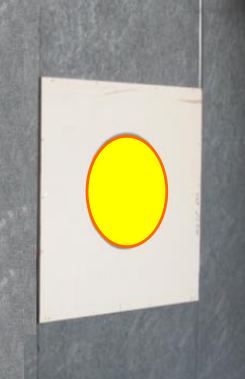
\includegraphics[width=5.0cm]{resources/wall-drilling}
  \caption{Picture of example target to drill out.}
  \label{fig:Wall-image}
\end{figure}

\newpage

% -------------------------------------------------------------------------------------
% RUBBLE CLEARING INTRO
%
\section*{Rubble Clearing Task}
\begin{enumerate}
\item Identify the location of the rubble/door using robot/human judgement from robot perception feedback.
\item Walk to the rubble and face it using the hubo\_walk panel.
\item Begin static balancing and squat to height which allows picking up rubble items.
\item Use dual-arm teleoperation to pick up the pieces of rubble and toss them to the side.
\end{enumerate}
\begin{figure}[h]
  \centering
  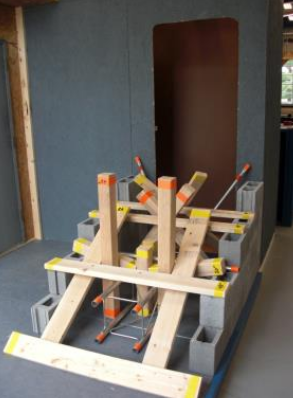
\includegraphics[width=5.0cm]{resources/rubble-clearing}
  \caption{Picture of example rubble scene.}
  \label{fig:Rubble-image}
\end{figure}

\newpage

% -------------------------------------------------------------------------------------
% INSTRUCTIONS
%
\section*{Operation Instructions}
\subsection*{Starting up Hubo}
\begin{enumerate}
  \item ssh hubo@192.168.0.201
  \item Turn on motor controllers with remote
  \item sudo service hubo-motion start
  \item launch RViz
    \begin{itemize}
    	  \item roscore
    	  \item rosrun rviz rviz
    \end{itemize}
  \begin{figure}[h]
    \centering
    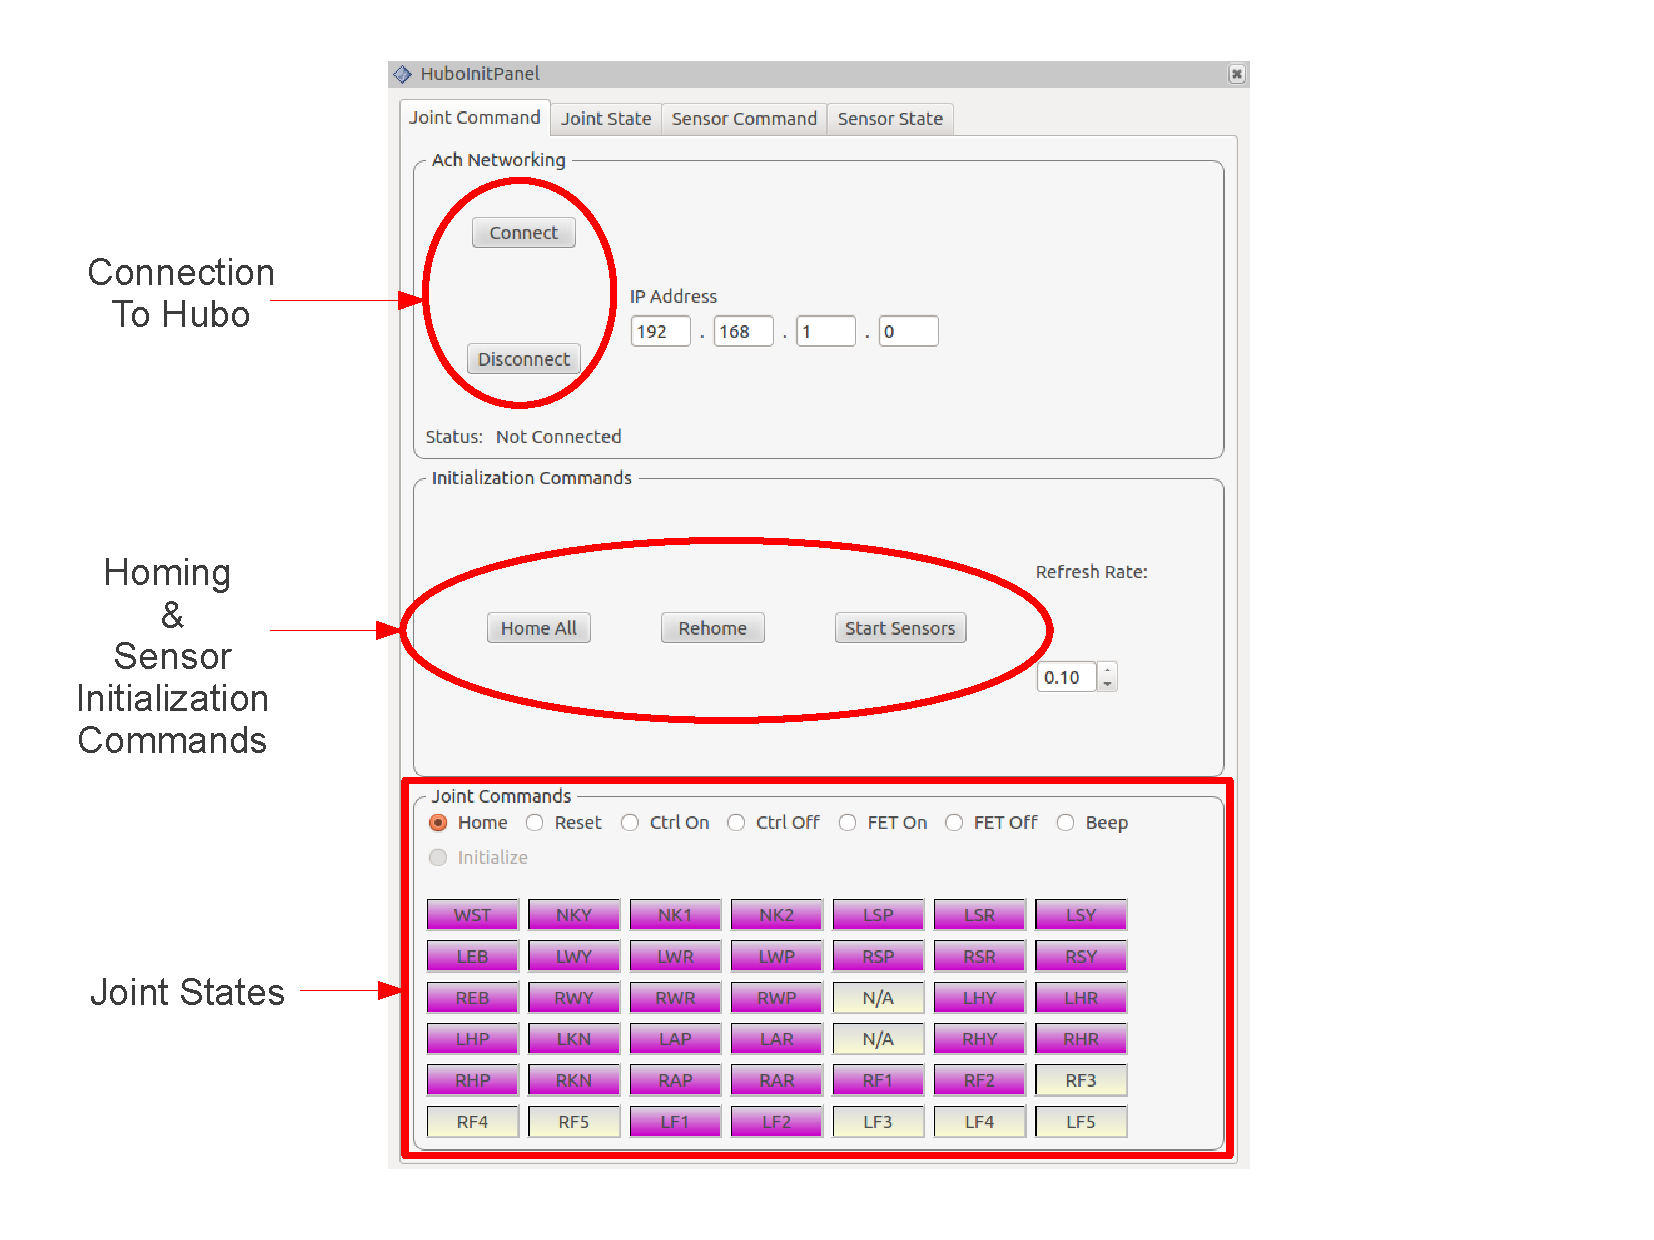
\includegraphics[width=15.0cm]{resources/hubo-init.pdf}
    \caption{Picture of hubo\_init panel.}
    \label{fig:hubo-init-image}
  \end{figure}
  \item Ensure "IP Address" is correct.
  \item Click "Connect" to push and pull ach channels between Hubo's computer and the remote computer.
  \item Click "Home All" to home all of Hubo's joints, if not on the ground and not homed. If already homed and standing, continue skip to step.
  \item If any active joints do not home, indicated by the color in the \textit{Joint State} section not being gray.
\end{enumerate}

% -------------------------------------------------------------------------------------
% TROUBLESHOOTING
%

% -------------------------------------------------------------------------------------
% REFERENCES
% -------------------------------------------------------------------------------------
%\bibliography{}

% -------------------------------------------------------------------------------------
% END DOCUMENT
% -------------------------------------------------------------------------------------
\end{document}
